\chapter{数据模型初探}

数据本身只反映出现象,因此我们的目的不仅仅是搜集数据本身,而是通过数据发现背后的机理和规律——
不只是回答“怎么样”,更重要的是回答“为什么”。而发现数据中规律的重要方法就是数据模型。

\section{交通流模型}

以一条道路上的交通状态为例,我们可以用流量$q$、密度$k$、速度$v$三个指标来描述。
其中根据物理守恒定律很容易推导出$q=k\cdot v$,另一方面密度$k$和速度$v$之间的关系就不是那么直观了。对于这种未知的关系,我们可以用一个函数$v=f(k)$表示,$f$的数学定义就代表了速度和密度之间的关系,也是路段上交通状态变化的背后机理。

为了找出合适的函数$f$我们要从实际出发,首先通过各种手段实际观测道路上的流量、密度、速度。
直接从现实世界观测到的数据称为\emph{实测数据(empirical data)}%
\sidenote{empirical是一个哲学词汇,反义词是ideological。分别表示基于现实世界的的和基于意识形态的证据}
,大量数据如果以数字表格形式存在,我们很难理解。
因此第一步一般是将数据可视化,绘制成某种图形。

路段流密速数据一般可视化方法是以将每一条记录画作一个数据点,横坐标表示密度、纵坐标表示速度或流量。实测数据绘制后一般呈现出类似\cref{fig:empirical-qkv}的形态,从中马上可以看出一些规律。
例如从左图中速度和密度之间的关系,可以看出随着密度增加速度总体呈下降趋势;而且密度较小时速度下降不明显。从右图中流量和密度之间的关系,可以看出随着密度增加流量呈先上升后下降的趋势。

\begin{figure*}
    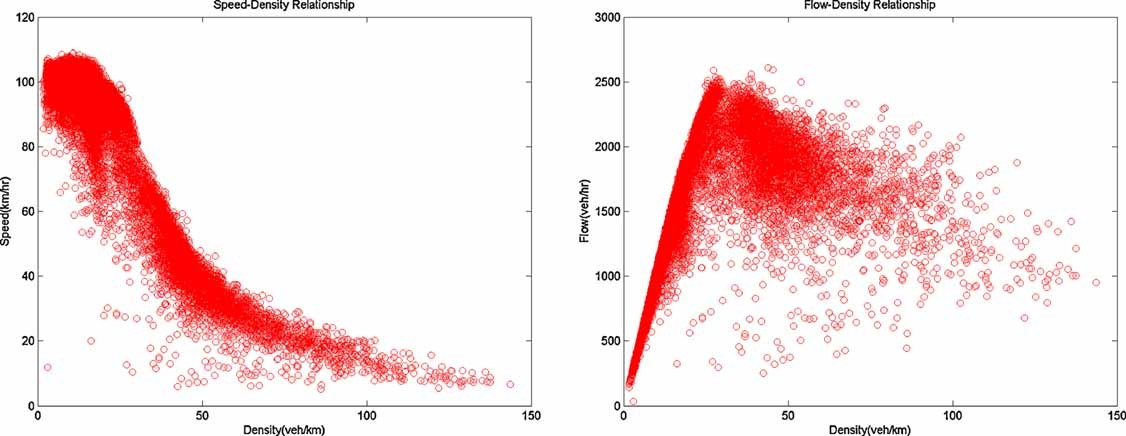
\includegraphics[width=\linewidth]{images/empirical-qkv.jpg}
    \caption{路段流量、密度、速度的典型实测数据}
    \label{fig:empirical-qkv}
\end{figure*}

由于我们已经知道$q=k\cdot v$,也就是说知道$k$,$v$就能计算出$q$,因此流量$q$对于我们来说是\emph{冗余数据(redundant data)},在后续分析中可以舍弃\sidenote{冗余数据并非没有价值,可以用于验证数据有效性。这里直接舍弃是为了简化讨论。}。此时我们面临的问题是,定义一个函数
\begin{equation}
    v=f(k)
\end{equation}
让该函数的图像与实测数据尽量符合,在数学上称为\emph{拟合问题}。

为了确定函数$f$的定义我们需要回答两个问题。第一个问题是函数的基本形态是什么?例如是直线、抛物线、还是指数曲线。这里我们假设$f$的图像是一条直线\sidenote{合理选取函数形式要综合考虑很多因素,没有标准答案,需要结合经验和对数据本身的理解。}
,也可以说$f$是\emph{线性函数}。
对于线性函数我们可以写出公式
\begin{equation}\label{eq:linear-kv}
    v = a\cdot k + b
\end{equation}
其中$a$和$b$是未知\emph{参数(parameter)}。
解析几何告诉我们$a$,$b$参数取值决定直线的形态,因此第二个个问题是$a$、$b$取值多少函数$f$与实测数据吻合\emph{最好}。

\section{线性回归}
为了确定\cref{eq:linear-kv}中的参数$a$、$b$我们需要用到一种叫做\emph{线性回归}的数学方法。
不过在正式介绍线性回归前,我们可以看一个简化的例子,方便理解为什么需要线性回归。

\subsection{线性方程}

假设我们实测的数据只有两组,即两个不同时刻的密度和速度,分别写作$p_1\coloneqq(k_1, v_1), p_2\coloneqq(k_2, v_2)$\sidenote{数学符号$\coloneqq$表示两边定义等价,读作“定义为”。}
,其中$p$代表数据点(point)。
此时图上只有两个数据点,函数$f$的图像是一条直线,显然当它同时穿过$p_1$、$p_2$时对数据的拟合最好。如何确定此时$a$、$b$的取值?

我们可以通过线性方程组来求解$a$、$b$。由于直线穿过两个数据点,以下两个方程必定成立:
\begin{equation}
    \left\{
    \begin{aligned}
        v_1 &= a\cdot k_1 + b \\
        v_2 &= a\cdot k_2 + b
    \end{aligned}\right.
\end{equation}
其中$a$、$b$是需要求解的未知数,可以用高斯消元法求解。
但这里我们先不求解,而是先把方程组写成线性代数的形式,方便后面的讨论。
首先将未知数写成单独分离,得到
\begin{equation}\label{eq:la-kv}
    \begin{bmatrix}
        v_1\\
        v_2
    \end{bmatrix}=
    \begin{bmatrix}
        k_1 & 1\\
        k_2 & 1
    \end{bmatrix}\cdot
    \begin{bmatrix}
        a\\
        b
    \end{bmatrix}
\end{equation}

可以看到方程由三项构成,我们分别规定用字母表示。其中左边是所有速度数据构成的向量%
\sidenote{注意区别$\vec{v}$和$v$,黑体字母$\vec{v}$表示向量,正常字母$v$表示标量。}
,写作$\vec{v}$;中间是一个权重(weight)矩阵,写作$\mat{W}$;右边是由所有参数构成的矩阵,写作$\vec{u}$。此时\cref{eq:la-kv}进一步简化表示为
\begin{equation}
    \vec{v}=\mat{W}\cdot\mat{u}
\end{equation}
如果权重矩阵$\mat{W}$可逆,参数$a$、$b$可以通过以下公式计算
\begin{equation}\label{eq:la-eq}
    \begin{bmatrix}
        a\\
        b
    \end{bmatrix}=
    \vec{u}=\mat{W}^{-1}\cdot\vec{v}
\end{equation}
而这里的权重矩阵$\mat{W}=\big[
\begin{smallmatrix}
    k_1 & 1\\
    k_2 & 1
\end{smallmatrix}$\big]
是$2\times2$的正方形矩阵,一般来说可逆。

\subsection{最小二乘法}

现在我们重新做了一次测量,得到一组新的数据$p_3\coloneqq(k_3, v_3)$,此时问题的性质发生了变化。按照上一节的步骤我们得到线性方正组
\begin{equation}\label{eq:la-kv-3}
    \begin{bmatrix}
        v_1\\
        v_2\\
        v_3
    \end{bmatrix}=
    \begin{bmatrix}
        k_1 & 1\\
        k_2 & 1\\
        k_3 & 1
    \end{bmatrix}\cdot
    \begin{bmatrix}
        a\\
        b
    \end{bmatrix}
\end{equation}
但是此时权重矩阵的尺寸是$3\times2$,一般来说不可逆,无法求解$a$,$b$。
无法求解的原因是我们有两个未知量$a$、$b$,但是有三个约束条件分别来自数据$p_1$、$p_2$、$p_3$,这类问题在数学上称为\emph{过约束}问题。

线性回归是解决这类过约束问题的常见方法,能够在没有精确解的情况下求出最优近似解。
当线性方程组$\vec{v}=\mat{W}\cdot\mat{u}$因为过约束无解时,方程两边同时乘以$\mat{W}^{-1}$,将\cref{eq:la-eq}转化为以下\emph{最小二乘形式}
\begin{equation}\label{eq:least-square}
    \mat{W}^{-1}\vec{v}=\mat{W}^{-1}\mat{W}\cdot\mat{u}
\end{equation}
此时方程是否有解由矩阵$\mat{W}^{-1}\mat{W}$是否可逆决定。
可以证明无论$\mat{W}$是什么形状,$\mat{W}^{-1}\mat{W}$都是正方形矩阵,一般来说可逆。
最佳近似解,为了与精确解区别记作$\hat{\mat{u}}$\sidenote{$\hat{\vec{u}}$读作"hat u"},可以通过以下公式计算
\begin{equation}
    \hat{\vec{u}}=(\mat{W}^{-1}\mat{W})^{-1}\mat{W}^{-1}\vec{v}
\end{equation}

\section{线性回归原理}

\cref{eq:least-square}中我们直接给出了线性回归求解最佳近似解的方法,本节将解释为什么这个公式有效。要理解线性回归的原理,有代数和几何两个角度。其中代数角度的关键是残差平方和最小,几何角度的关键是向量空间的正交投影。以下将分别解释。

\subsection{残差平方和最小}
假定参数$a$,$b$为已知量,利用\cref{eq:linear-kv}可以根据密度$k$计算速度$v$。
此时一个密度对应两个速度,一个称为\emph{实测值}另一个称为\emph{预测值}。
例如密度$k_1$对应的实测值是$v_1$,预测值为了区别记作$\hat{v}_1=f(k_i)=ak_1+b$。
实测值和预测值之间的差别称为\emph{残差},记作$e_1=\hat{v}_1-v_1$。
理想情况下实测值与预测值吻合,残差$e_1=0$;如果做不到,越接近$0$越好。

\subsubsection{残差平方和}

当有多个数据点时,我们需要一个指标表示所有数据点预测值和估计值的总体吻合程度,常用的指标\emph{残差平方和(Sum of Squares Error)}定义为:
\begin{equation}\label{eq:sse}
    \text{SSE}=\sum_{i=1}^n {e_i}^2=\sum_{i=1}^n (v_i-f(k_i))^2
\end{equation}
其中$n$是数据点数量,$e_i$代表第$i$个数据点的残差。残差平方和并不是唯一的指标,首先介绍的原因是他有一些良好的性质,可以简化数学处理。
另一个常用的指标是\emph{残差绝对值之和}$\sum_{i=1}^{n}|e_i|$,虽然在数学处理上难度更高,但是在其他方面更有优势,会在后续章节介绍。

根据以上定义可以看出残差平方和$\text{SSE}$是参数$a$、$b$的函数,因为不同的$a$、$b$取值会影响预测值$\hat{v}$,进而影响到残差$e_i$,再而影响到残差平方和。需要特殊强调这个函数关系时残差平方和可以记作$\text{SSE}(a,b)$或者$\text{SSE}(\vec{u})$,接下来我们推导它的公式。

根据\cref{eq:sse}的定义,我们可以把残差平方和写成向量\emph{点积}形式
\begin{equation}\label{eq:sse-vec}
    \begin{split}
        \text{SSE}&=\sum_{i=1}^n {e_i}^2=
        \begin{bmatrix}
            e_1 & e_2 &\cdots & e_n
        \end{bmatrix}
        \cdot
        \begin{bmatrix}
            e_1 \\
            e_2 \\
            \vdots\\
            e_n
        \end{bmatrix}\\
        &=\vec{e}^T\cdot\vec{e}
    \end{split}
\end{equation}
其中$\vec{e}=[\begin{smallmatrix}
    e_1 & e_2 & \cdots & e_n
\end{smallmatrix}]^T$是所有残差构成的列向量。
接下来我们写出残差向量$\vec{e}$的公式
\begin{equation}\label{eq:e-vec}
    \begin{split}
        \vec{e}=
        \begin{bmatrix}
            e_1 \\
            e_2 \\
            \vdots\\
            e_n
        \end{bmatrix}&=
        \begin{bmatrix}
            v_1 \\
            v_2 \\
            \vdots\\
            v_n
        \end{bmatrix}-
        a\cdot
        \begin{bmatrix}
            k_1 \\
            k_2 \\
            \vdots\\
            k_n
        \end{bmatrix}-
        b\cdot
        \begin{bmatrix}
            1 \\
            1 \\
            \vdots\\
            1
        \end{bmatrix}\\
        &=\vec{v}-a\vec{k}-b\vec{1}\\
        &=\vec{v}-\mat{W}\vec{u}
    \end{split}
\end{equation}
其中$\vec{v}$是所有速度实测值的向量,$\mat{W}$是权重矩阵,$\vec{k}$是所有密度数据的向量,$\vec{1}$是全$1$向量。

把\cref{eq:e-vec}带入\cref{eq:sse-vec},然后展开化简可以得到
\begin{equation}
    \begin{split}
        \text{SSE(a,b)} &= \vec{e}^T\cdot\vec{e}\\
        &=(\vec{v}-\mat{W}\vec{u})^T(\vec{v}-\mat{W}\vec{u})\\
        &=\vec{v}^T\vec{v}+(\mat{W}\vec{u})^T\mat{W}\vec{u}
        -\vec{v}\mat{W}\vec{u}-(\mat{W}\vec{u})^T\vec{v}\\
        &=\vec{v}^T\vec{v}+\vec{u}^T\mat{W}^T\mat{W}\vec{u}
        -\vec{v}\mat{W}\vec{u}-\vec{u}^T\mat{W}^T\vec{u}
    \end{split}
\end{equation}